\section{Factor Graphs}

For problems that include many variables influencing each other it is useful to have an abstract representation of how those	 variables are related to each other. So called factor graphs are such representations.\newline

In general, factor graphs represent the structure of a function's factorization into smaller functions. \newline If a function $f(X_1, \ldots, X_n)$ can be written as a product $\prod_{j=1}^{m}{f_j(S_j)}$  where the functions $f_j$ have smaller inputs $S_j \subset X$, its factorization 
can be expressed by a factor graph: The graph has two types of nodes: 
\emph{variable nodes} that correspond to the variables $X_i$ and \emph{factor nodes} corresponding to the functions $f_j$. An edge connects a variable node $X_i$ to a factor node $f_j$ if $X_i$ is part of $f_j$'s input. 
This means the factor graph is an undirected bipartite graph with the node set $ V = \{X_1, \ldots, X_n\} \cup \{f_1, \ldots, f_n\}$ and edge set $E = \{(X_i, f_j) \; | \; X_i \in S_j\}$. 

In many applications the global function $f$ is a joined probability distribution that can be factorized by using information about independence between the variables. Typical tasks on factor graphs are computing variable assignments that maximize or minimize $f$ or computing marginal distributions if $f$ is a probability distribution. Both of these will be done in Section \ref{BPFS}\newline

\begin{example}
For random variables $X_1, X_2 \text{ and } X_3$ their joined probability distribution $f$ is defined as $f(x_1, x_2, x_3) := P(X_1 = x_1 \land X_2  = x_2 \land X_3 = x_3)$. If $X_2$ and $X_3$ are conditionally independent given $X_1$ this function can be factorized: $$f(x_1, x_2, x_3) = P(X_1 = x_1) * P(X_2 = x_2 \land X_3 = X_3 \; | \; X_1 = x_1)$$
This factorization still contains a factor depending on all variables. If $X_2$ and $X_3$ are known to be conditionally independent given $X_1$ this factor can again be factorized:

$$f(x_1, x_2, x_3) = \underbrace{P(X_1 = x_1)}_{f_1(x_1)} * \underbrace{P(X_2 = x_2 \; | \; X_1 = x_1)}_{f_2(x_1, x_2)} * \underbrace{P(X_3 = x_3 \; | \; X_1 = x_1)}_{f_3(x_1, x_3)}$$

%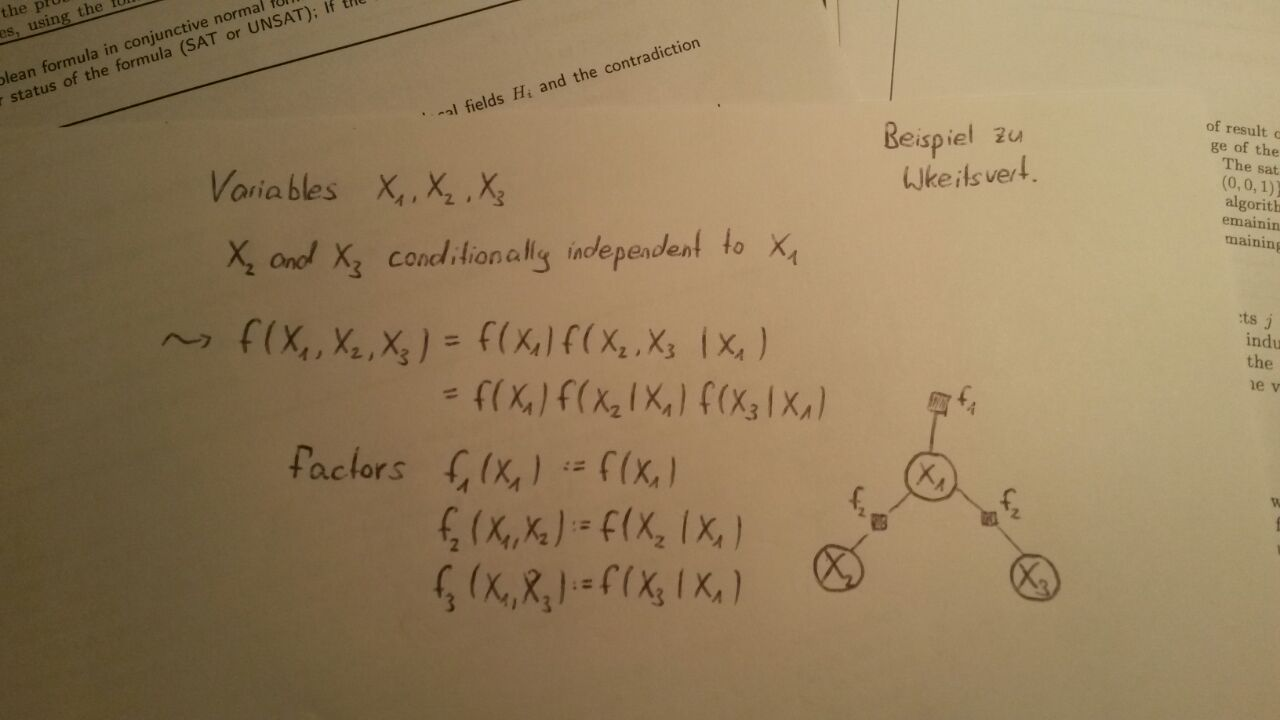
\includegraphics[scale = 0.3]{img/Proba1}
\begin{figure}
\centering

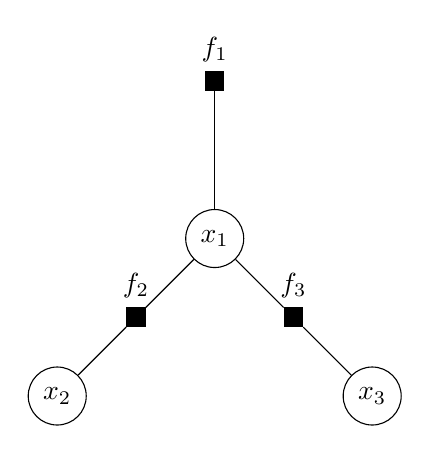
\begin{tikzpicture}[scale=1.0,transform shape]
   	\node[shape=circle,draw=black] (x1) at (0,0) {$x_1$};
    \node[shape=circle,draw=black] (x2) at (-2,-2) {$x_2$};
    \node[shape=circle,draw=black] (x3) at (2,-2) {$x_3$};
    \node[rectangle,draw=black, label = {$f_1$}, fill] (f1) at (0,2) {};
    \node[rectangle, fill, draw=black, label = {$f_2$}] (f2) at (-1,-1) {};
    \node[rectangle, fill, draw=black, label = {$f_3$}] (f3) at (1, -1) {} ;

    \path [-] (x1) edge node[left] {} (f1);
    \path [-] (x1) edge node[left] {} (f2);
    \path [-] (x1) edge node[left] {} (f3);
    \path [-] (f2) edge node[left] {} (x2);
    \path [-] (f3) edge node[left] {} (x3);
   
\end{tikzpicture}
\caption{Factor graph of $f$s factorization into $f_1, f_2, f_3$}
\end{figure}

the variable nodes are drawn here as circles whereas constraint nodes are drawn as rectangles to easily distinguish the types of nodes

\end{example}
% zu allgemein?
%
%A Constraint Satisfaction Problem (\textit{CSP}) consists of a set of variables $X = \{x_1, \ldots, x_n\}$, a set of domains $D = \{D_1, \ldots, D_n\}$ that specify which values each variable may take and a set of constraints $C = \{C_1, \ldots, C_m\}$ that must hold for the chosen values $x_i \in D_i$. \newline
%SAT can be written as CSP where each clause $C_j = {x_i, \ldots, x_k}$

%\newtheorem*{definition}{Definition}
\newpage
Factor graphs can also be used for describing constraint satisfaction problems. A factor corresponds to a constraint on its neighbour vertices, it evaluates to $1$ if the constraint is satisfied and to $0$ if not. For the global function $f$ - the product of all factors - to be $1$, every constraint has to be is satisfied. The special case of SAT problems is discussed in the following chapter.



\subsection{Factor graph of a SAT Problem}
A SAT formula in CNF form can be interpreted as a boolean function that factorizes to the formulas clauses. \newline
In the corresponding factor graph each factor node $a$ represents the local function defined by a single clause of the original formula. The clause is a disjunction of variables and negated variables $(x_i\lor \overline{x_j} \lor \ldots)$. If the variable $x_i$ or its negation $\overline{x_i}$ appears in this clause the factor graph contains an edge between $a$ and the variable node $i$.

In \cite{survprop} some additional notation is defined to simplify the description of the algorithms in section \ref{PBFS}: 
\begin{definition} Let $a$ be a factor node and $i$ a variable node
\begin{itemize}
\item The value $J_i^a$
\end{itemize}
\end{definition}
The constraints can directly be viewed as functions ...


\begin{example}
$$F = \underbrace{(x_1 \lor x_2 \lor x_3)}_{a} \land \underbrace{(\overline{x_1} \lor x_3 \lor x_4) }_{b}\land \underbrace{(\overline{x_3} \lor x_4)}_{c} \land \underbrace{(\overline{x_1} \lor \overline{x_2})}_{d}$$

The defined values of clause $n$ are $V_+(b) = \{x_2, x_4\}, V_-(b) = \{x_1\}$

\begin{figure}[h]
\centering

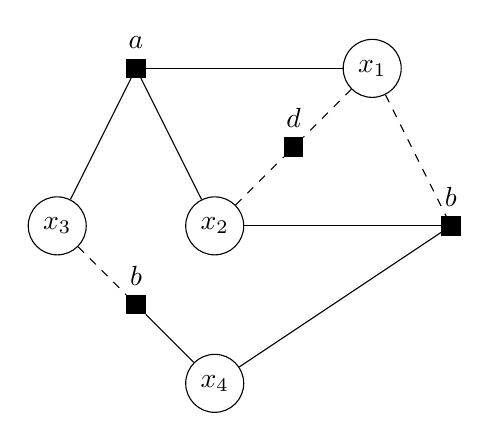
\begin{tikzpicture}[scale=1.0,transform shape]
   	\node[shape=circle,draw=black] (x1) at (3,0) {$x_1$};
    \node[shape=circle,draw=black] (x2) at (1,-2) {$x_2$};
    \node[shape=circle,draw=black] (x3) at (-1,-2) {$x_3$};
    \node[shape=circle,draw=black] (x4) at (1,-4) {$x_4$};
    
    \node[rectangle,draw=black, label = {$a$}, fill] (a) at (0,0) {};
     \node[rectangle,draw=black, label = {$d$}, fill] (d) at (2,-1) {};
     \node[rectangle,draw=black, label = {$b$}, fill] (b) at (4,-2) {};
     \node[rectangle,draw=black, label = {$b$}, fill] (c) at (0,-3) {};
     
 
    \path [-] (x1) edge node[left] {} (a);
    \path [-] (x2) edge node[left] {} (a);
    \path [-] (x3) edge node[left] {} (a);
    
    \path [dashed] (x1) edge node[left] {} (d);
    \path [dashed] (x2) edge node[left] {} (d);
    
    \path [-] (x2) edge node[left] {} (b);
    \path [dashed] (x1) edge node[left] {} (b);
    \path [-] (x4) edge node[left] {} (b);
    
    \path [-] (x4) edge node[left] {} (c);
    \path [dashed] (x3) edge node[left] {} (c);
    

  
\end{tikzpicture}
\caption{Factor graph of a SAT formula}
\end{figure}

Again the circles are variable nodes, the rectangles are constraint nodes. If if $x_i$ appears negated in the clause $a$ (if $J_a^i = 1$), the edge is drawn dotted.  

\end{example}
